\documentclass[12pt, oneside]{article} 
\usepackage[english]{babel}
\usepackage[T1]{fontenc}
\usepackage{graphicx}	
\usepackage{lscape}
\usepackage{booktabs}
\usepackage{array}
\usepackage{amsmath}
\usepackage{amssymb}
\usepackage{enumitem}
\usepackage{caption}
\usepackage{subcaption}
\usepackage{setspace}
\usepackage{epstopdf}
\usepackage{float}
\usepackage{rotating }
\usepackage{rccol}
\usepackage{tikz}
\usepackage{ctable}
\usepackage{dsfont}
\usepackage{longtable}
\usepackage{tabto}
\usepackage[flushleft]{threeparttable}
\usepackage[toc,page]{appendix}
\usepackage{multicol}
\usepackage{color}
\usepackage{fancyhdr}
%\usepackage{hyperref} % for links in the table of contents
\usepackage[inner=2.3cm, outer=2.3cm, top=2.55cm, bottom=2.8cm]{geometry} % pour modifier les marges
\usepackage{setspace}
\usepackage{parskip}
\bibliographystyle{plain}
\usepackage{url}

\begin{document}

\begin{titlepage}
  \begin{center}
    

\huge
\textbf{University of Zurich}
\vspace{0.5cm}

\textbf{Digital Tools for Finance:}

\textbf{Report}

\rule{\textwidth}{1pt}
\vspace{1cm}
\large

\textbf{Bastien Tognolini: 21-409-925 }
\vspace{0.5cm}

\textbf{Nicolas Profumo: 19-419-290 }
\vspace{0.5cm}

\textbf{Lucille Dauer: 20-205-670 }
\vspace{0.5cm}

\textbf{Pierre Nicolas Angevin: 19-823-921}




  \end{center}



\end{titlepage}

\begin{center}
\tableofcontents
\end{center}
\newpage


%-------------------------------------------------------------------------------------------
%	INTRODUCTION
%-------------------------------------------------------------------------------------------
\section{Introduction}
Stock markets are events of constant influence, building up investor expectations, and one of the most closely watched is product announcements. Such announcements introducing advanced technology, or an innovative solution might generally have an immediate effect in the financial world through share price movements. For companies like Apple and Samsung, which are known for products that have defined the industry, such moments are a part of their valuation and investor confidence.

This project tries to investigate the relationship between major product announcements and stock volatility for leading technology companies, focusing on the market's responsiveness in the days before and after events. By using historical data derived from key announcements, we try to explore patterns of price fluctuations and volatility to get a good view of the market's response to new information and understand how investors and companies could use this methodology in their decisions.


Our motivation comes with the dual challenge of analyzing investor behavior and the applicability of digital tools to real-life financial analysis. With the development of skills in programming and data science, one can now dissect large datasets, identify patterns, and confirm hypotheses with an unprecedented degree of accuracy. In addition, this study explores the way product announcements affect stock prices and serves as a practical training in these tools.


This paper describes the methodology to be followed in data collection and analysis, pinpoints the challenges faced in the same, and presents the results based on financial data about the top 10 largest market capitalization of technological companies. It develops a broad sense of perspectives on how corporate events affect the stock market and adds to knowledge in improving the understanding of financial market dynamics. Also, this research, through these findings, tries to throw some light on how market behavior changes with product announcements and adds value to academicians and practising investors.



\section{Data}

\subsection{Data Importation, Merging and Cleaning}
Initially, we prepared and imported all the necessary data to set up foundation for our analysis. We gathered all the data in two separated Excel files.
The first one was compiled with Refinitiv EIKON (Datastream) that gathers daily stock prices in USD (adjusted for dividends) from 31.12.2013-31.12.2023 for the ten biggest tech firms in terms of current market capitalization. The second one was retrieved by ChatGPT and contains the product announcement dates and their related product names for each firm of the above-mentioned list. However, because we did not know if we could fully trust ChatGPT, we randomly checked five announcement dates for different firms.

Finally, we chose to sort the data by company and dates in order to facilitate the computations of the daily stock returns. We ended up with a dataset where each row contains a company name, a given date, a daily stock price and a product name if one was announced on this day.


\subsection{Compute Daily Returns \& Rolling Volatility}
Having our merged and cleaned dataset, we computed the daily stock returns and rolling volatility over a 10-day window. Due to the way we chose to build our dataset, we had to perform those computations separately for each company. Then, we also had to delete the missing values due to the fact that the first row of each stock can't provide a daily return and that the 10 day rolling volatility can't be computed before having 10 data points. Therefore, we had to check that the sum of the missing values for the "Daily\_Return" and "Rolling\_Volatility" columns were respectively 10 and 100. Finally, after getting rid of this nan values we obtained our final dataset such as shown-below.

\begin{table}[ht]
    \centering
    \resizebox{\textwidth}{!}{%
        \begin{tabular}{llcccc}
            \toprule
            \textbf{Name} & \textbf{Date} & \textbf{Announcement} & \textbf{StockPrice} & \textbf{Daily\_Return} & \textbf{Rolling\_Volatility} \\
            \midrule
            AMZN & 2014-01-14 & NaN & 20299.90 & 0.016778 & 0.010152 \\
            AMZN & 2014-01-15 & NaN & 20214.63 & -0.004201 & 0.010226 \\
            AMZN & 2014-01-16 & NaN & 20211.05 & -0.000177 & 0.010216 \\
            AMZN & 2014-01-17 & NaN & 20405.61 & 0.009626 & 0.010606 \\
            AMZN & 2014-01-20 & NaN & 20405.61 & 0.000000 & 0.010248 \\
            \bottomrule
        \end{tabular}%
    }
    \caption{Sample of the final dataset}
    \label{tab:final dataset}
\end{table}


\section{Descriptive Analysis}

\subsection{Descriptive Statistics of the Daily Returns}
First, we grouped the data by the "Name" column, which represents the different firms, allowing us to compute the relevant statistics for each firm individually. The analysis focused on the "Daily\_Return" column, which measures the percentage change in stock prices on a daily basis. 

Using this grouped data, we computed several key metrics. These included the mean daily return, expressed as a percentage, which reflects the average performance of the firm's stock over the last 10 years. We also calculated the standard deviation of the daily returns. Additionally, we identified the minimum and maximum daily returns, which represent the worst and best performing days in the last 10 years for each firm, respectively. 

\begin{table}[ht]
    \centering
    \begin{tabular}{lcccc}
        \toprule
        \textbf{Name} & \textbf{Mean (\%)} & \textbf{Std (\%)} & \textbf{Min (\%)} & \textbf{Max (\%)} \\
        \midrule
        AMZN  & 0.100 & 2.055 & -14.049 & 14.131 \\
        APPL  & 0.109 & 1.758 & -12.865 & 11.981 \\
        AVGO  & 0.151 & 2.156 & -19.913 & 15.834 \\
        GOOG  & 0.077 & 1.727 & -11.634 & 16.259 \\
        META  & 0.098 & 2.315 & -26.390 & 23.283 \\
        MSFT  & 0.112 & 1.675 & -14.739 & 14.217 \\
        NVDA  & 0.230 & 2.872 & -18.756 & 29.807 \\
        TECHY & 0.070 & 2.189 & -12.418 & 23.261 \\
        TSLA  & 0.186 & 3.447 & -21.063 & 19.895 \\
        TSMC  & 0.091 & 1.617 & -8.870  & 10.337 \\
        \bottomrule
    \end{tabular}
    \caption{Descriptive Statistics of the Daily Returns  by firm}
    \label{tab:returns_stats}
\end{table}


As we can observe in Table 2, Nvidia and Tesla have the highest average daily performances with respectively 0,230\% and 0,186\% which seems coherent from a risk-return trade-off perspective because they also have the highest risk with respective volatility of 2,879\% and 3,447\%. However, we notice that Nvidia performed better than Tesla but is on average less volatile which is inconsistent with the risk-return trade-off. Finally, we noticed a negative asymmetry of the returns for Apple, Broadcom (AVGO), Meta, Microsoft and Tesla. However, half of the firms doesn't show the same pattern in the distribution of their extreme returns which goes against the general idea that returns are negatively skewed.

\subsection{Cumulative Performance Analysis}
Let's now take a look at the cumulative performance of each firm over the last 10 years. As we can see on Figure 1 below, the cumulative performance of Nvidia over the last 10 years is astonishing compared to the other firms. Indeed, a small increase in the average daily return implies an exponential increase of the cumulative performance over the last 10 years due to the compounding effect. 

We found this graph very interesting because the AI trend is pretty recent but we can observe that Nvidia began to over-perform the other firms back in 2017. However, back at the time Nvidia wasn't such the giant that it is today so it might not be relevant to compare it with the other firms at that time as they probably all had very different market capitalizations and return expectations as they have today.

\begin{figure}[H]
    \centering
    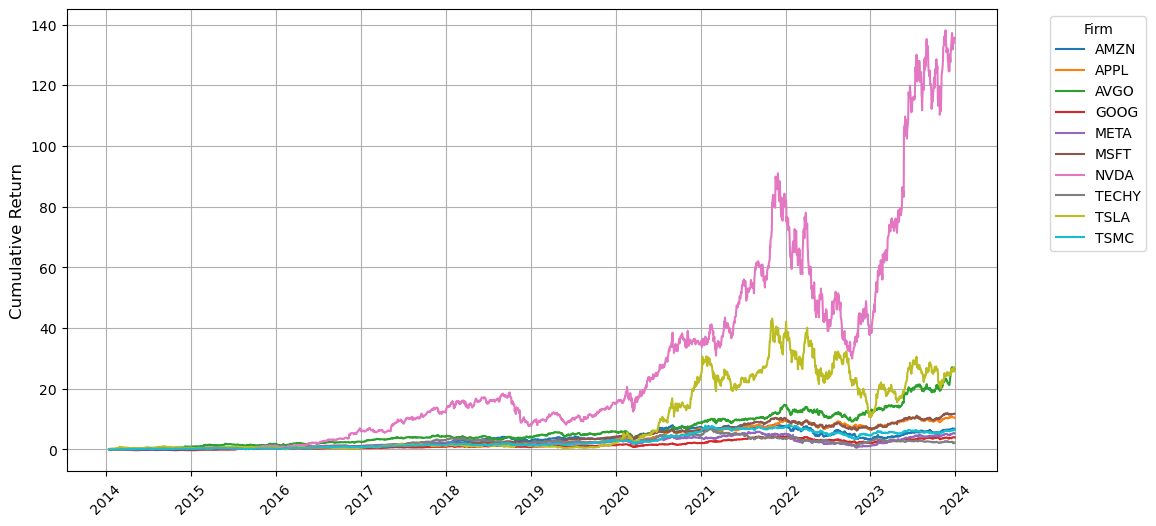
\includegraphics[width=0.8\linewidth]{../images/cum_perf_analysis.png}
    \caption{Cumulative Performance by firm}
    \label{fig:cum_perf}
\end{figure}


\subsection{Volatility Analysis}
Now, let's try to look at the rolling volatility computed on a 10 day window to illustrate the risk-return tradeoff. As we can see on Figure 2 below, there is of course no free lunch on financial markets. Indeed, greater performance comes with greater risk and we can observe that the volatility of Tesla and Nvidia are almost always above the others. We can spot the Covid Crisis on the graph in early 2020 and we can see a spike of volatility for every firms during this period.

\begin{figure}[H]
    \centering
    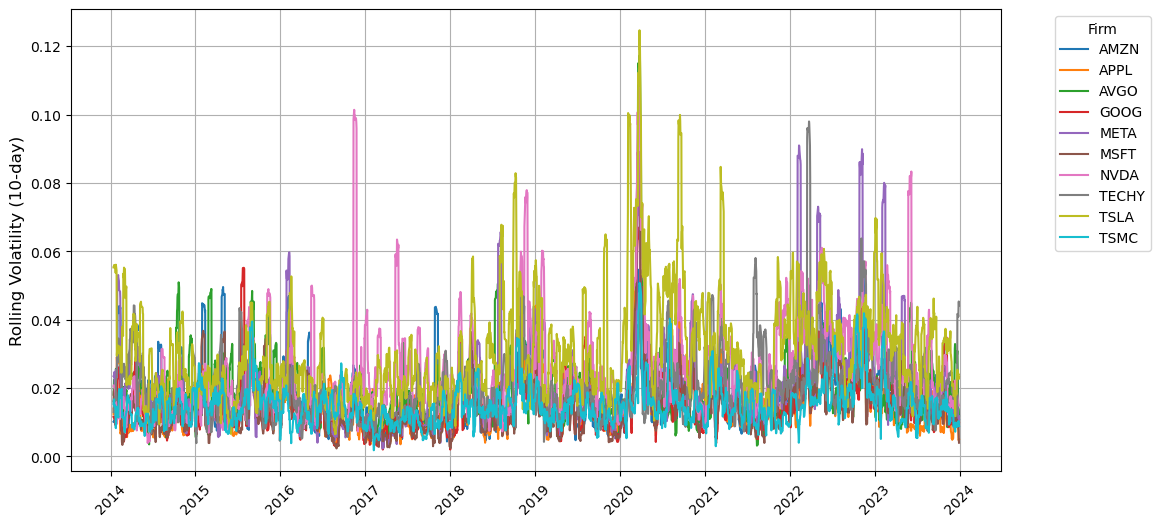
\includegraphics[width=0.8\linewidth]{../images/volatility_analysis.png}
    \caption{Volatility over Time by firm}
    \label{fig:volatility_analysis}
\end{figure}

An interesting pattern is the spikes of volatility for Nvidia in the 2016-2017 period. In fact, we can see that at the end of 2016, the volatility of the AI giant surged while the others were relatively low. This could coincide with major AI improvements and the donation of the first AI supercomputer in August 2016 by Jensen Huang to Elon Musk which was working back at the time for a well-known startup today, OpenAI. In 2022, OpenAI gave open access to its virtual assistant chatbot, ChatGPT, which helped to popularize AI among the public. It could imply that back at the time, Nvidia was becoming, also thanks to its new Pascal Architecture, a leader in Artificial Intelligence and that the stock volatility surged because investors were already anticipating the potential growth of the company in the upcoming years.

\subsection{Spotting Patterns between Volatility and Product Announcements}

\subsubsection{Looking for patterns at the 10 year horizon}
In this section, we will try to spot patterns between Volatility and Product Announcements within our dataset. Let's begin by looking for a potential impact of product announcements on the rolling volatility of the GAFAM firms. We only focus on those firms for readability purpose but we could choose any other subsets or even all firms in the dataset.

\begin{figure}[H]
    \centering
    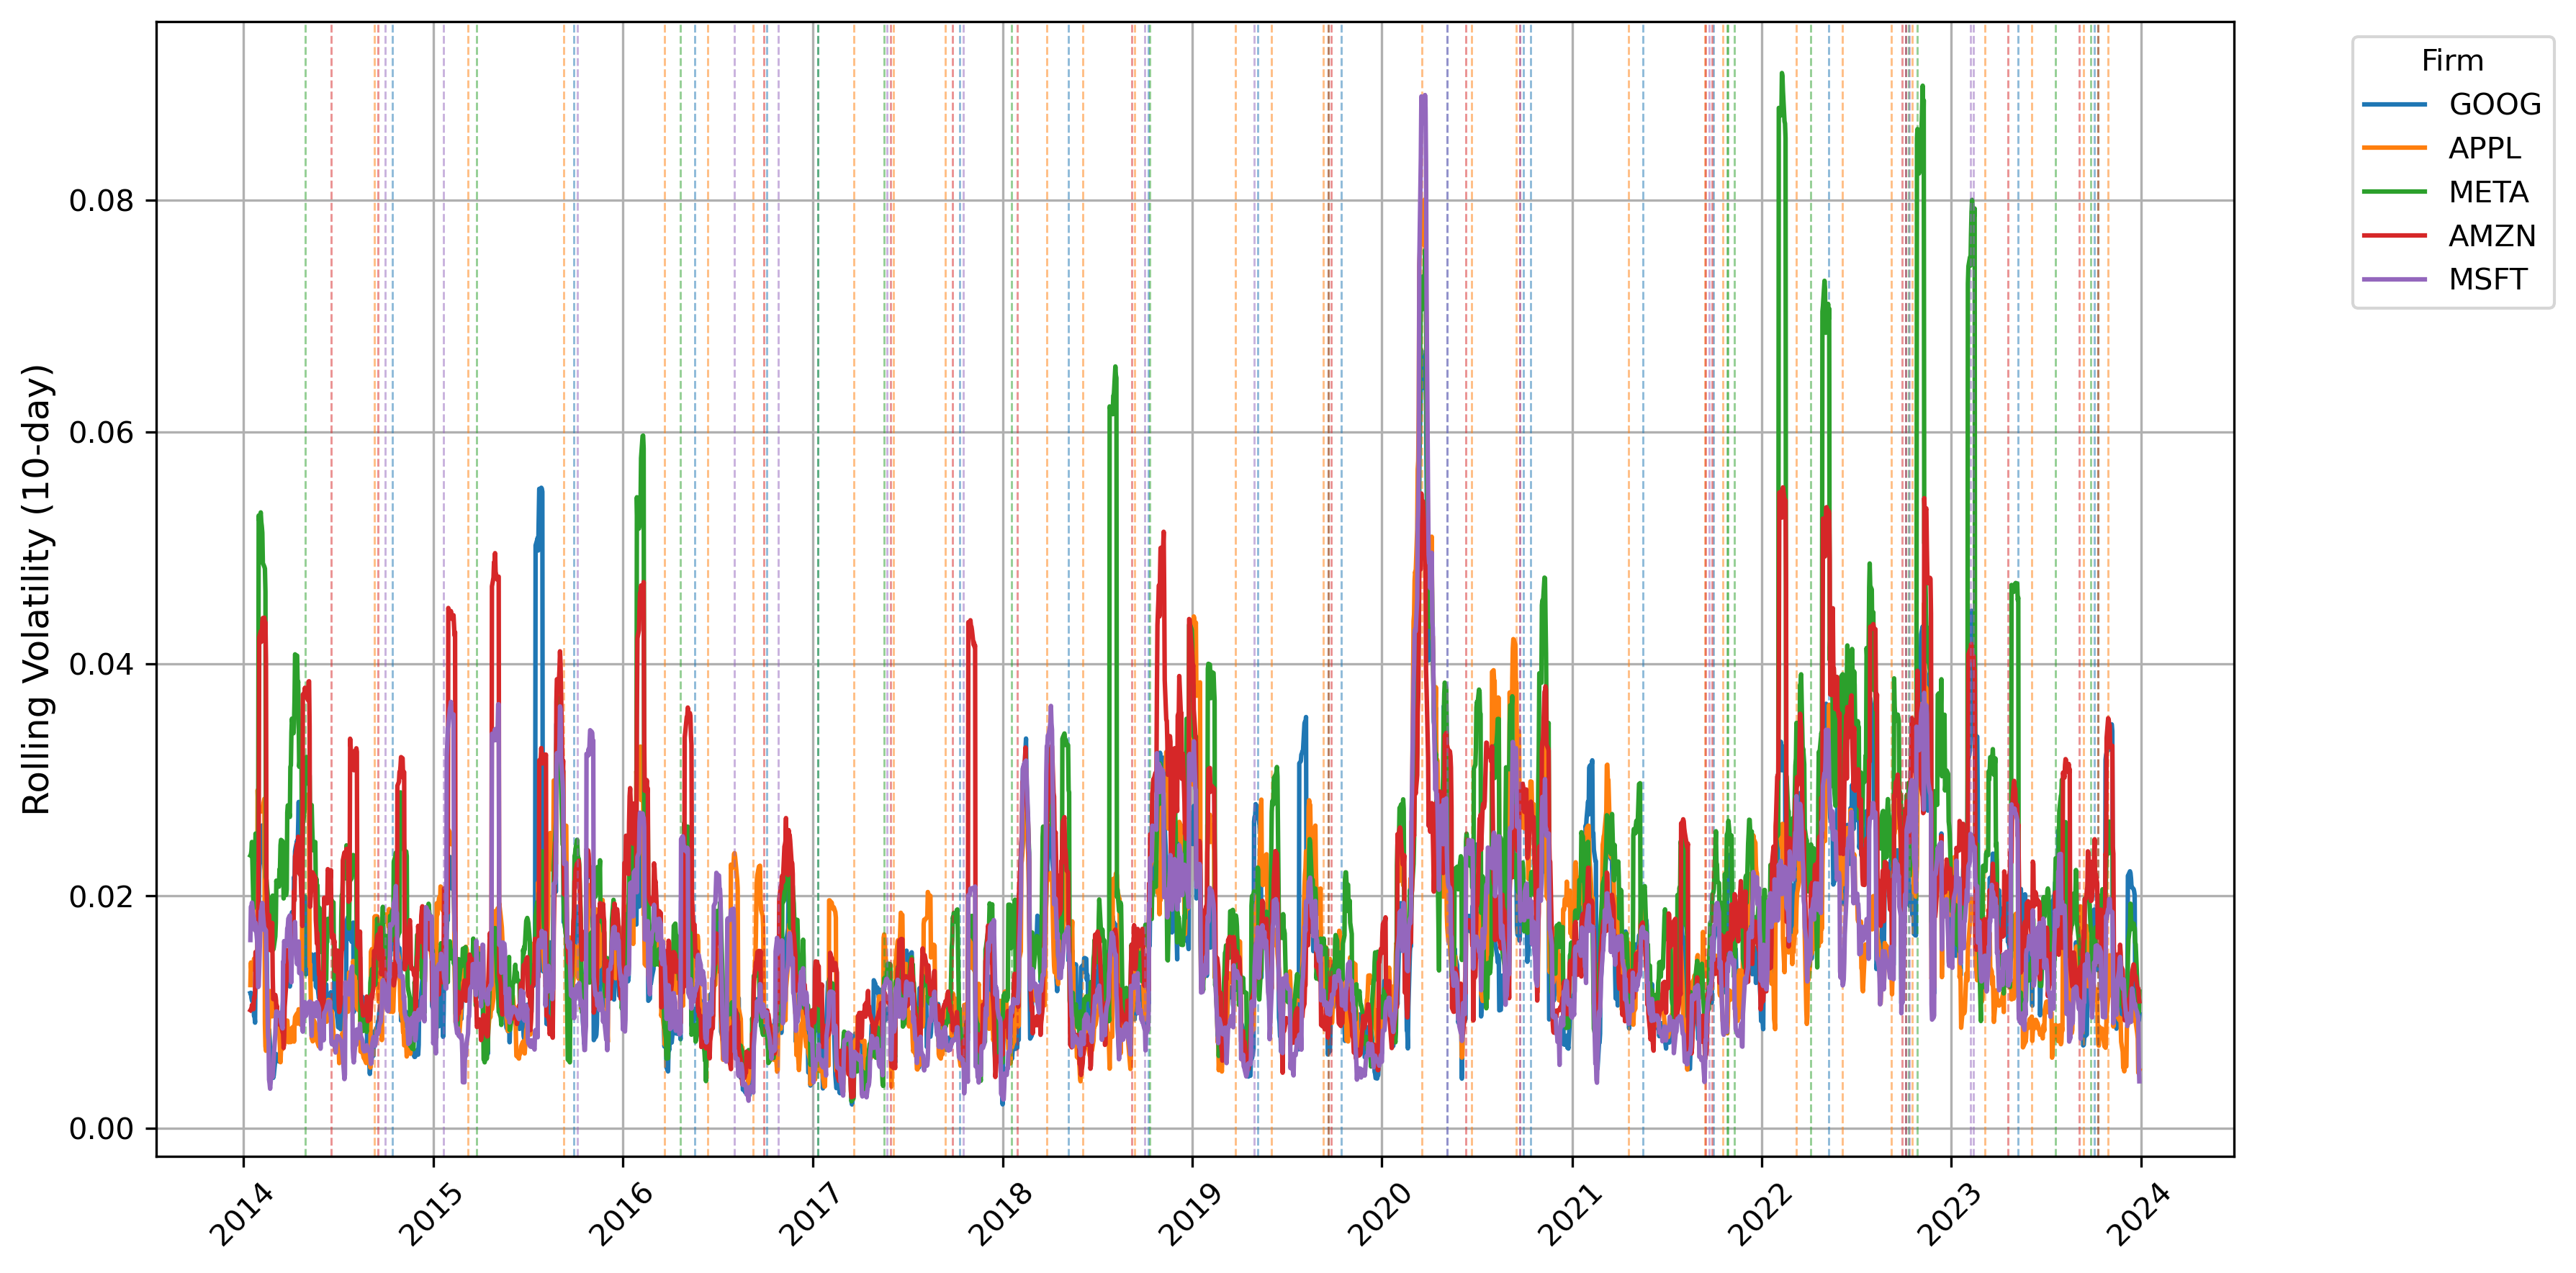
\includegraphics[width=0.8\linewidth]{../images/GAFAM_pattern.png}
    \caption{Volatility and Product Announcements for GAFAM}
    \label{fig:GAFAM_pattern}
\end{figure}

By observing Figure 3, there doesn't seem to be a clear relationship between product announcements (represented by a dashed line of the same colour of the firm it was announced by) and the computed 10 day rolling volatility which is not very surprising because we are looking at the 10 year horizon, making it difficult to spot any correlations between our 2 variables of interest. Additionally, the rolling window methodology will just shift from one day and give a weight of 1/10 to the additional return computed on the product announcement date making it hard to have a lot of impact on the overall measure except in case of extreme fluctuations.

Therefore, the product announcements does not seem to have many effects on the volatility at first sight which forced us to try to focus on specific time frames or firms in the following sections.

\subsubsection{Looking for patterns on a shorter time horizon for a specific firm}
Now, we will look for a potential relationship between the volatility and product announcement for a specific firm (Google in our case) and for a specific time-frame (the Covid Crisis)

We plotted the rolling volatility of Alphabet Inc. (GOOG) stock between 2019 and 2020. The data was filtered to focus on GOOG stock for the specified years, and the rolling volatility was plotted over time to observe trends and variations. Key announcement dates were highlighted on the plot with vertical dashed lines along with their related product names, offering additional context to understand how these events may have influenced volatility. This visualization provides a concise representation of volatility trends alongside significant announcements, illustrating potential market responses to key events. 

\begin{figure}[H]
    \centering
    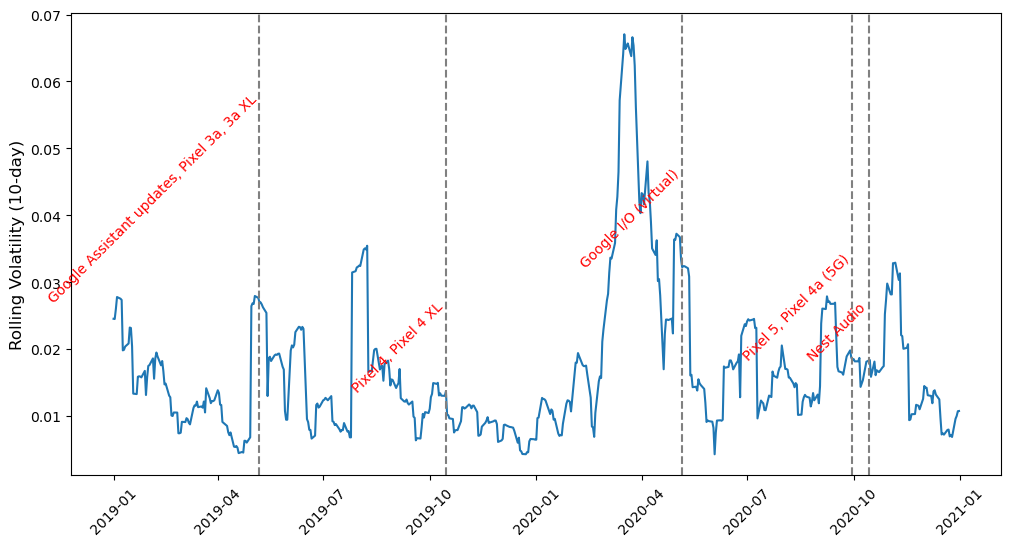
\includegraphics[width=0.8\linewidth]{../images/GOOG_pattern.png}
    \caption{Volatility and Product Announcements during COVID crisis for Google}
    \label{fig:GOOG_pattern}
\end{figure}

By observing Figure 4, we can see the volatility spike due to the Covid Crisis but the product announcement doesn't seem to have a systematic impact on the rolling volatility. Consequently, despite our initial intuition that product announcements necessarily have an effect on the stock volatility, such a pattern does not clearly emerge from our dataset. Therefore, we will try to refine the analysis once again.

\subsubsection{Looking for patterns on a daily basis for a specific TESLA Product}
Finally, we try to focus on a specific product (Tesla Model S P85D) from a specific firm (Tesla) within a very short specific time frame around the annoucement date (30 days).

\begin{figure}[H]
    \centering
    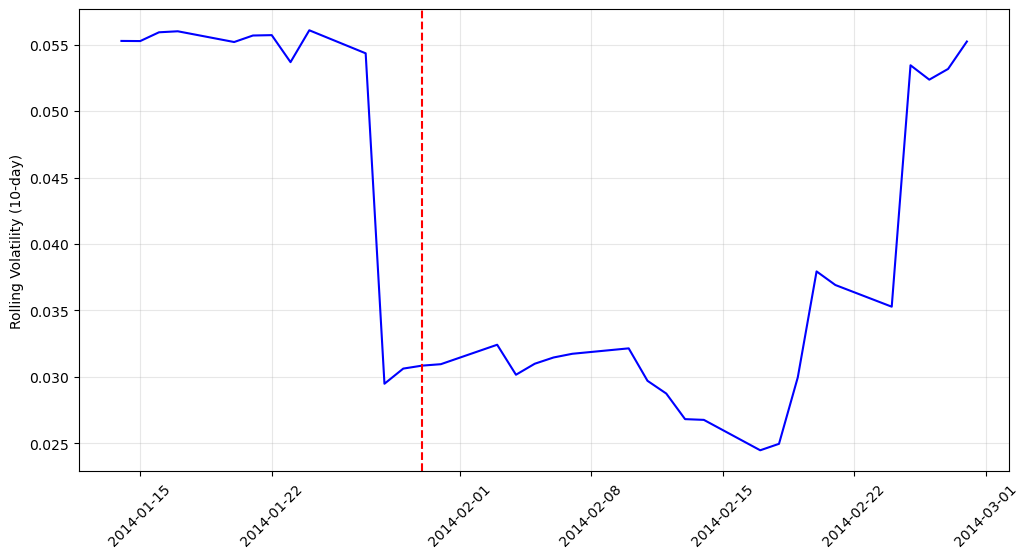
\includegraphics[width=0.8\linewidth]{../images/TESLA_pattern.png}
    \caption{Tesla Stock Volatility around Model S P85D Announcement}
    \label{fig:TESLA_pattern}
\end{figure}

By observing Figure 5, we noticed a counterintuitive pattern that seems to indicate a decrease in volatility when the Tesla Model S P85D was announced. This could maybe due to the extreme volatile behavior of the Tesla stock where investors would be reassured by the product announcement but it goes against financial intuition  and Tesla stock was not that volatile back in 2014 so we will not hazard ourselves into such reasoning.

To conclude, we managed to observe interesting patterns within our dataset, but we did not identify clear volatility spikes around the announcement dates. This suggests that other factors beyond product announcements could be more influential in driving volatility or that we could have used different volatility measures or time horizons. We will further develop this point in the Conclusion section.

\section{Model}
The final step involved testing the statistical significance of the relationship between product announcements and stock volatility using the following linear regression analysis:

\[
\text{Rolling\_Volatility}_{it} = \alpha + \beta \cdot \text{Announcement}_{it} + \epsilon_{it}
\]

We created a binary variable to represent announcement days (1 for announcement days, 0 for non-announcement days) and used rolling volatility as the dependent variable. The dataset was then split into training and testing sets. Indeed, 20\% was used for training and 80\% to assess the accuracy of the model. Without even looking at the results, we can already say that this model is very naive and does not include any control variables to avoid potential bias due to omitted variables. Furthermore, we already know that there is too few announcement dates which will imply that the coefficients of the regression will not be significant.

\section{Results}
The regression output reveals the following: The intercept is 0.019317 (1.93\%), representing the average level of rolling volatility. The coefficient is 0.001916 (0.19\%), indicating a positive (as expected) but not significant effect of announcements on volatility. The R² score is -0.0005099, suggesting a very poor model fit, indicating that the average rolling volatility is a better predictor than our model.
\begin{table}[ht]
    \centering
    \begin{tabular}{lc}
        \toprule
        \textbf{Parameter} & \textbf{Value} \\
        \midrule
        Intercept & 0.019317437887891822 \\
        Coefficient for Announcement\_Binary & 0.0019166839158981386 \\
        R\(^2\) Score & -0.0005099587924510818 \\
        \bottomrule
    \end{tabular}
    \caption{Regression Results}
    \label{tab:regression_outputs}
\end{table}


As expected, the analysis reveals a weak or non-existent linear relationship between product announcements and the rolling daily volatility computed on a 10 days window. It appears that product announcements alone might not predict stock volatility effectively and implies that the relationship might be more complex than a simple linear model. Our visual insights further support these conclusion (cf. Spotting patterns sections). The time series plot, with vertical lines marking announcement dates, does not show a consistent pattern of volatility spikes around these events. This suggests that other factors, beyond product announcements, might also play a role in driving stock volatility.

However, keep in mind that the poor quality of the model might also come from other factors such as the small number of observations for the independent variable, the choice of the volatility measure and the difficulty to find relevant control variables.


\section{Conclusion}
In conclusion, product announcements alone do not appear to significantly impact stock volatility. The relationship between announcements and volatility is either non-existent or too complex (non-linear for example) to capture with a simple linear model. Future research should consider additional factors and employ more sophisticated analytical approaches to better understand this relationship.

\subsection{Limitations \& Future Improvements}
Firstly, we definitely believe there is an impact of the product announcement on the stock volatility but it is hard to know where it exactly takes place: for example, is it when the product is announced or released? Indeed, there might be rumors, leaks or newspaper articles already influencing investors ahead of those official events.

Consequently, finding control variables that would be correlated with the product announcement and have an impact on the stock volatility is not an easy task and definitely not trivial. However, factors such as changes in interest rates, geopolitical events, and general economic conditions could have a significant impact on volatility and affect product announcements of firms: for example if there is an increase in interest rates, corporate loans become more expensive and there is less money for R\&D so less product announcements at the end for a given firm. Finally, considering time-based effects, such as seasonality, could also add depth to our analysis by capturing periodic fluctuations that may influence investor behavior.

Furthermore, we also think that the impact might be on the intra-day volatility of the stock but such data are not easy to retrieve. Then, it is also important to understand that the small number of observations related to product announcements contributed to make our model irrelevant and not significant. Indeed, there is an asymmetry between stock returns computed daily and products announced only several times in a year.

Additionally, the rolling volatility window size might also have an impact on the absence of correlation between our variables of interest. We could also have adjusted the measure by putting more weight on the most recent returns for example.

Finally, differences in the types of product announcements were not factored into our analysis, meaning that we treated all announcements as equal, even though their market impact could vary significantly. Finally, variations in company size, which could influence how announcements are received by the market, were not considered, potentially leading to skewed results.

\subsection{Business Implications}
Let's have a look at the business implications of this model. We see that for investors the results indicate that product announcements alone should not guide trading decisions. Investors need to consider a broader range of factors beyond announcements when evaluating stock price movements. The traditional adage of "buy the rumor, sell the news" may not apply in this context, as the impact of announcements on volatility is minimal.

If we have a look at the companies side the findings imply that product announcements do not significantly destabilize stock prices. This allows companies to focus on product strategy and innovation without excessive concern for short-term market reactions. Other factors, such as macroeconomic conditions or industry trends, may have a larger role in ensuring stock price stability.

In conclusion, this suggests that investors and companies should focus on broader market factors and fundamentals rather than individual announcement events when considering stock price volatility. The findings challenge the common assumption that major product announcements significantly affect stock behavior, emphasizing the importance of a more comprehensive approach when analyzing market dynamics.

\newpage
%-------------------------------------------------------------------------------------------
%	BIBLIOGRAPHY
%-------------------------------------------------------------------------------------------

\newpage
\nocite{*}
\bibliography{references}
\newpage
%-------------------------------------------------------------------------------------------


%----------------------------------------------------


\end{document}